\documentclass{beamer}
\usepackage{graphicx}
\usepackage{fancyvrb}
\usetheme{Berlin}

\defbeamertemplate*{background canvas}{custom-background}{
    
\includegraphics[width=\paperwidth,height=\paperheight]{background.png}
}

\usebackgroundtemplate{%
    
\includegraphics[width=\paperwidth,height=\paperheight]{background.png}
}

\title{Kubernetes CronJob Controller}
\author{avengeHERs}
\date{}

\begin{document}

\frame{\titlepage}

\section{Our Team}
\begin{frame}{Meet Our Team}
    \begin{columns}
        \column{0.33\textwidth}
        \begin{figure}
            \centering
            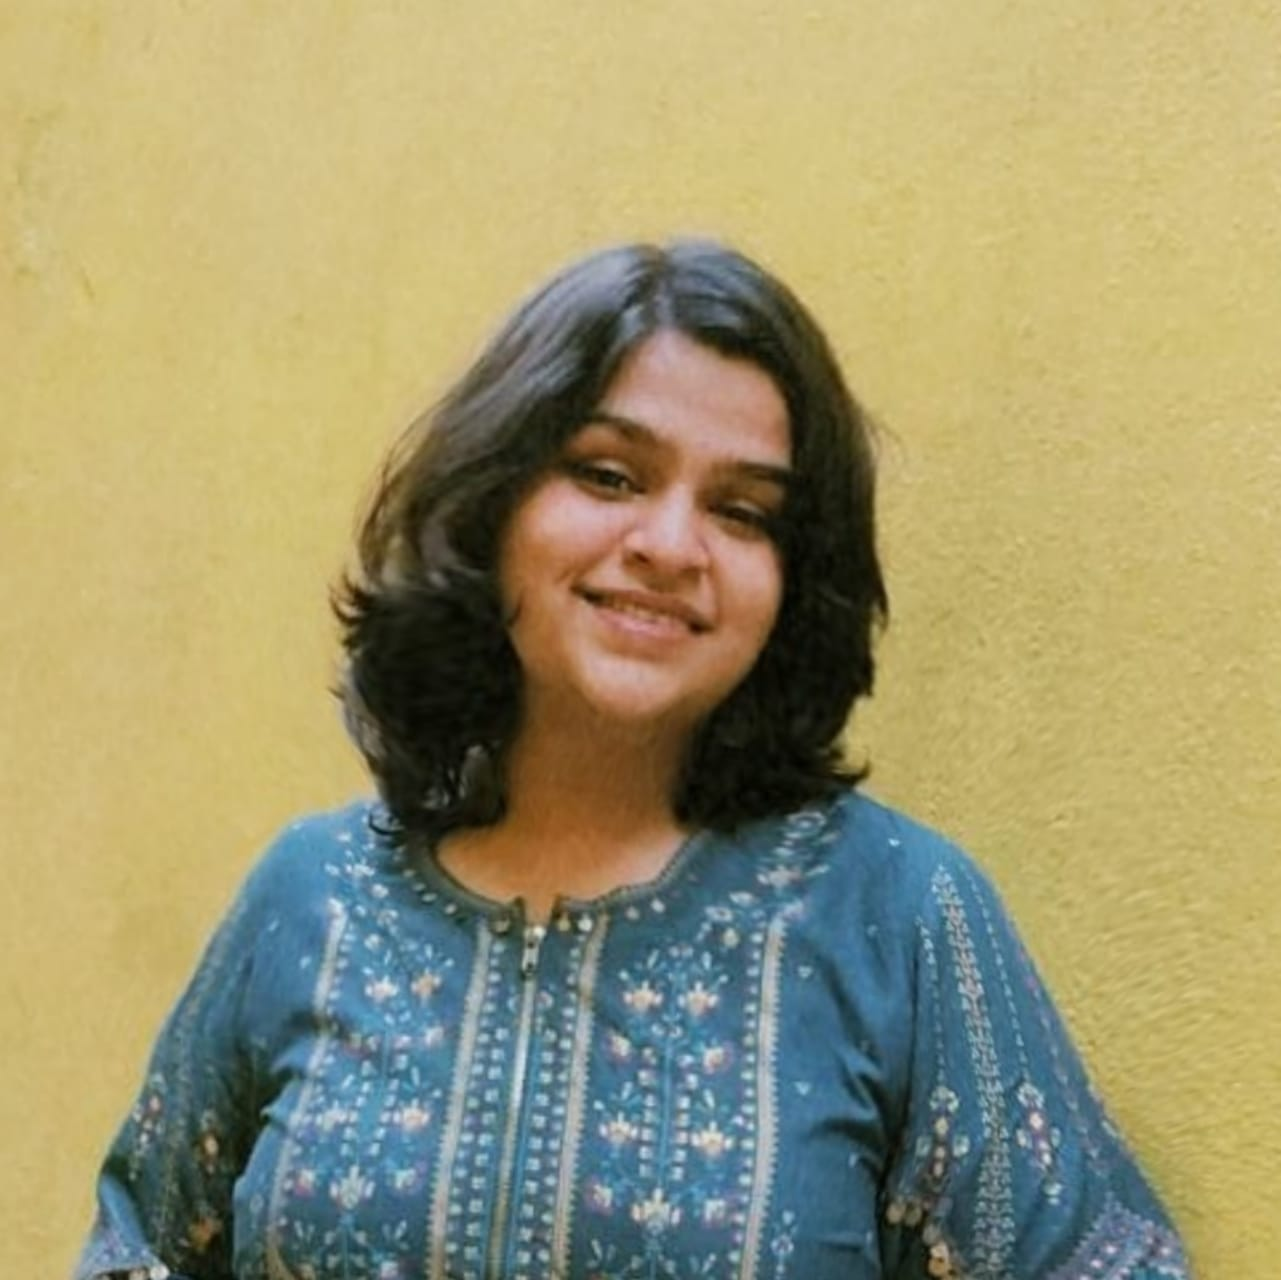
\includegraphics[height=3cm]{Srishti.jpg}
           Srishti Dutta
        \end{figure}
        
        \column{0.33\textwidth}
        \begin{figure}
            \centering
            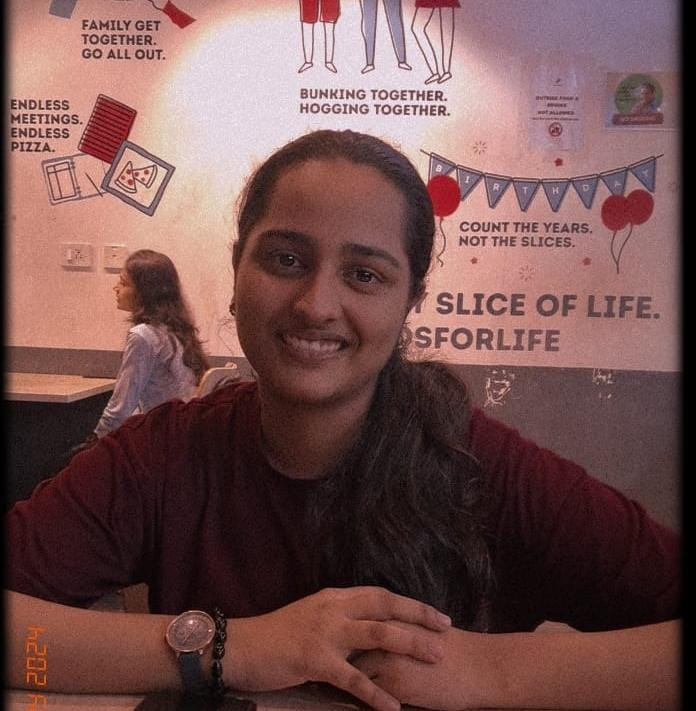
\includegraphics[height=3cm]{Meghna.jpg}
            Meghna Mandawra
        \end{figure}

        \column{0.33\textwidth}
        \begin{figure}
            \centering
            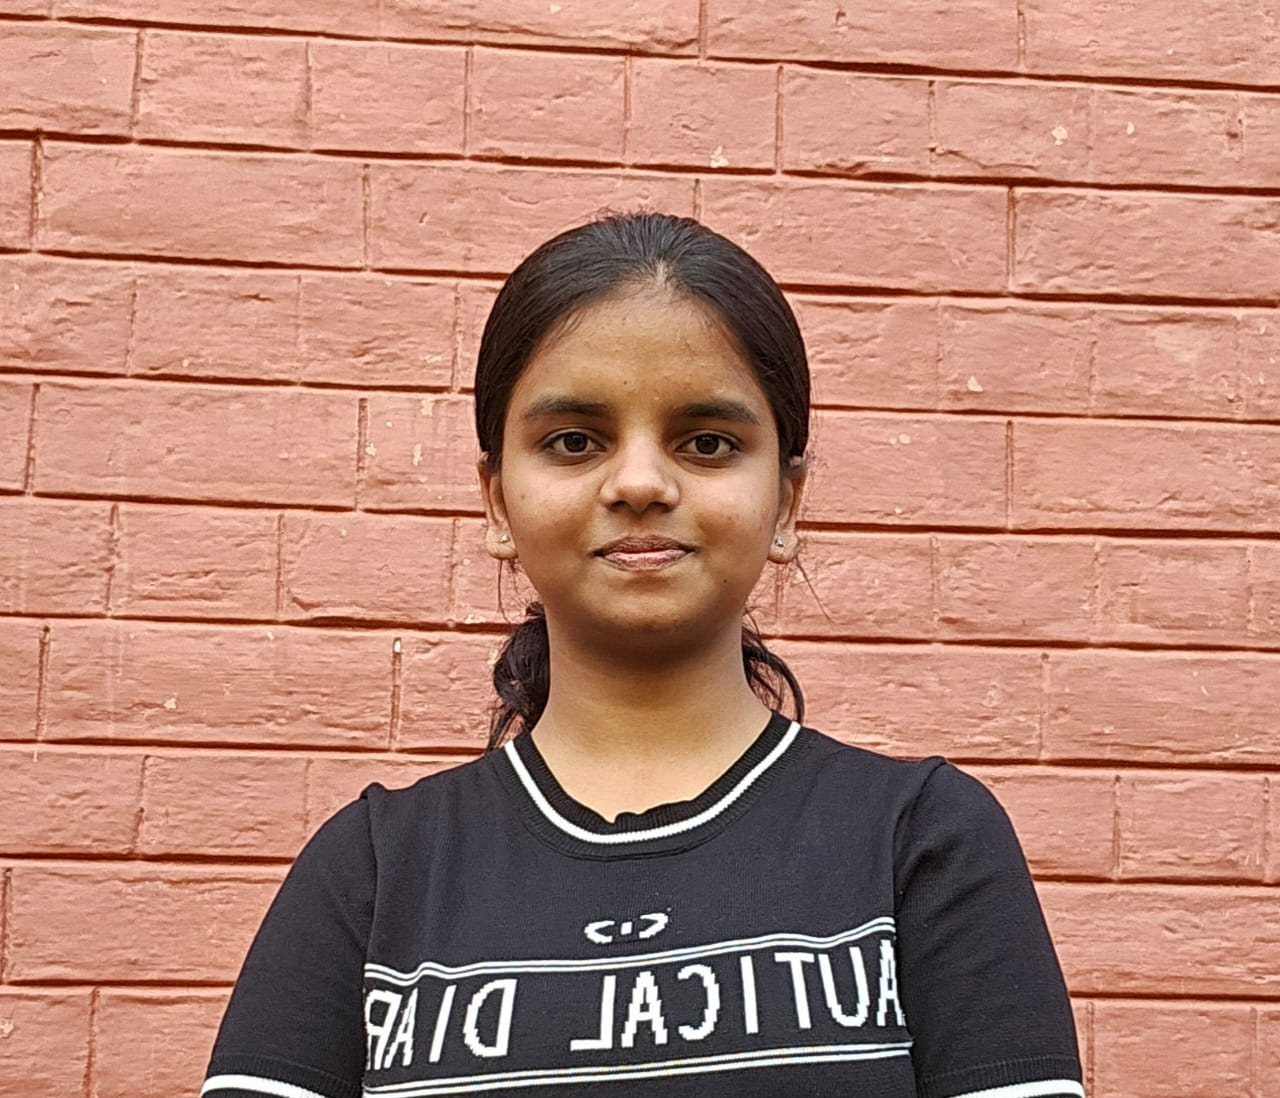
\includegraphics[height=3cm]{Khushi.jpg}
           Khushi S.
        \end{figure}
    \end{columns}
\end{frame}


\section{Introduction to Kubernetes}
\begin{frame}{What is Kubernetes?}
    \begin{itemize}
        \item Open-source platform for managing containerized applications.
        \item Developed by Google, now maintained by CNCF.
        \item Automates deployment, scaling, and management of containerized apps.
    \end{itemize}
\end{frame}

\section{Containerized Applications}
\begin{frame}{What are Containerized Applications?}
    \begin{itemize}
        \item Applications packaged with all dependencies.
        \item Ensures consistency across different environments.
        \item Commonly used containers: Docker, CRI-O, containerd.
    \end{itemize}
\end{frame}

\section{Why We Need Kubernetes}
\begin{frame}{Why Kubernetes?}
    \begin{itemize}
        \item Manages containerized applications at scale.
        \item Provides automated load balancing and resource management.
        \item Facilitates self-healing through automatic restart and rescheduling.
    \end{itemize}
\end{frame}


\section{Kubernetes Controllers}
\begin{frame}{Kubernetes Controllers}
    \begin{figure}
        \centering
        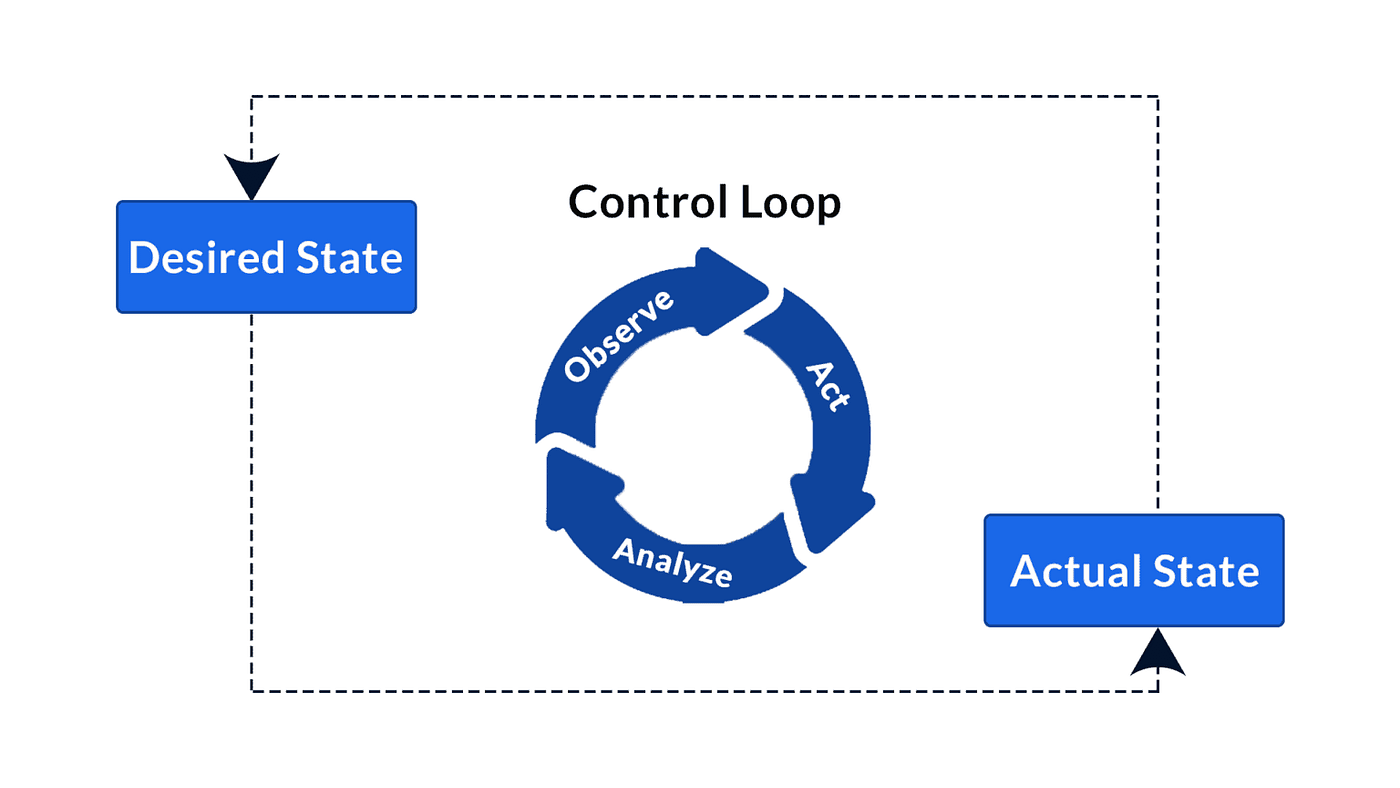
\includegraphics[width=0.5\textwidth]{controllers.png}
    \end{figure}
    \begin{itemize}
        \item Control loops that manage the state of the system.
        \item Ensure that the desired state matches the actual state.
        \item Examples: Deployment Controller, ReplicaSet Controller, CronJob Controller.
    \end{itemize}
\end{frame}

\section{Kubernetes CronJob Controller}
\begin{frame}{What is a CronJob Controller?}
    \begin{itemize}
        \item Manages time-based job scheduling.
        \item Runs jobs at specified times, similar to Linux cron.
        \item Useful for periodic tasks like backups, reports, etc.
    \end{itemize}
\end{frame}

\section{How the CronJob Controller Works}
\begin{frame}{How the CronJob Controller Works}
    \begin{figure}
        \centering
        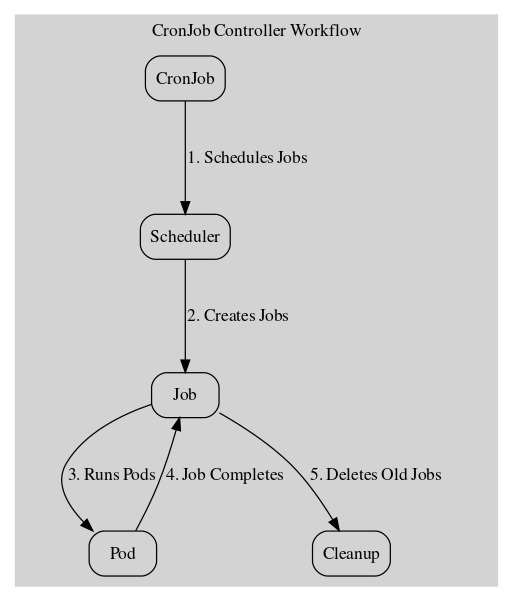
\includegraphics[width=0.5\textwidth]{cronjob.jpg}
    \end{figure}
\end{frame}
\section{How the CronJob Controller Works}
\begin{frame}{How the CronJob Controller Works}
    \begin{itemize}
        \item Watches for CronJob resources in the cluster.
        \item Reads the schedule defined in the CronJob.
        \item Creates a Job resource at the scheduled time.
        \item The Job resource runs the specified task by creating Pods.
        \item Marks the Job as successful or failed based on task completion.
        \item Cleans up old Job resources to manage cluster resources efficiently.
    \end{itemize}
\end{frame}

\section{Steps we followed to Build a CronJob k8s Controller}
\begin{frame}{Steps we followed}
    \begin{enumerate}
        \item \textbf{Set Up Environment:}
        \begin{itemize}
            \item Installed Kubernetes, Kubebuilder, and Go.
            \item Ensured all necessary tools were correctly configured.
        \end{itemize}
        \item \textbf{Created a New Project:}
        \begin{itemize}
            \item Used Kubebuilder to initialize a new project.
            \item Scaffolded the basic structure of the controller.
        \end{itemize}
        \item \textbf{Defined the CustomResourceDefinition (CRD):}
        \begin{itemize}
            \item Created a CRD for CronJob.
            \item Specified the API schema for the CronJob resource.
        \end{itemize}
        \item \textbf{Implemented Controller Logic:}
        \begin{itemize}
            \item Developed the reconciliation logic to manage CronJobs.
            \item Handled events like creation, updates, and deletions.
        \end{itemize}
       
        \item \textbf{Tested and Validated:}
        \begin{itemize}
            \item Ensured the controller ran and managed tasks correctly.
        \end{itemize}
    \end{enumerate}
\end{frame}

\section{Challenges Faced}
\begin{frame}{Challenges Faced}
    \begin{itemize}
        \item Issues integrating the controller into the cluster.
        \item Go environment uninstalls itself when the laptop is powered off, causing interruptions.
       \item Confusing documentation made it challenging to follow the setup and usage.
       \item The make command resulted in errors.
    \end{itemize}
\end{frame}

\section{Key Learnings}
\begin{frame}{Key Learnings}
    \begin{itemize}
        \item Gained a comprehensive understanding of Kubernetes.
        \item Improved Go programming skills.
        \item Enhanced troubleshooting and debugging skills - learned firsthand that it can lead to sleepless nights.
        \item Improved collaboration and communication within the team.
        \item Realized the value of perseverance over instant gratification.
    \end{itemize}
\end{frame}

\section{Thank You}
\begin{frame}{}

            fmt.Println("Thank You")
        
\end{frame}

\end{document}
